\documentclass[a5paper, 10pt]{article}

% Текст
\usepackage[utf8]{inputenc} % UTF-8 кодировка
\usepackage[russian]{babel} % Русский язык
\usepackage{indentfirst} % красная строка в первом параграфе в главе
% Отображение страниц
\usepackage{geometry} % размеры листа и отступов
\usepackage{listings}
\usepackage{color}

\geometry{
	left=12mm,
	top=25mm,
	right=15mm,
	bottom=17mm,
	marginparsep=0mm,
	marginparwidth=0mm,
	headheight=10mm,
	headsep=7mm,
	nofoot}
\usepackage{afterpage,fancyhdr} % настройка колонтитулов
\pagestyle{fancy}
\fancypagestyle{style}{ % создание нового стиля style
	\fancyhf{} % очистка колонтитулов
	\fancyhead[LO, RE]{Лабораторная работа № 2 } % название документа наверху
	\fancyhead[RO, LE]{Задачи 1296, 1494} % название section наверху
	\fancyfoot[RO, LE]{\thepage} % номер страницы справа внизу на нечетных и слева внизу на четных
	\renewcommand{\headrulewidth}{0.25pt} % толщина линии сверху
	\renewcommand{\footrulewidth}{0pt} % толцина линии снизу
}
\fancypagestyle{plain}{ % создание нового стиля plain -- полностью пустого
	\fancyhf{}
	\renewcommand{\headrulewidth}{0pt}
}
\fancypagestyle{title}{ % создание нового стиля title -- для титульной страницы
	\fancyhf{}
	\fancyhead[C]{{\footnotesize
			Министерство образования и науки Российской Федерации\\
			Федеральное государственное автономное образовательное учреждение высшего образования
	}}
	\fancyfoot[C]{{\large 
			Санкт-Петербург, 2024
	}}
	\renewcommand{\headrulewidth}{0pt}
}

% Математика
\usepackage{amsmath, amsfonts, amssymb, amsthm} % Набор пакетов для математических текстов
%\usepackage{dmvnbase} % мехматовский пакет latex-сокращений
\usepackage{cancel} % зачеркивание для сокращений
% Рисунки и фигуры
\usepackage[pdftex]{graphicx} % вставка рисунков
\usepackage{wrapfig, subcaption} % вставка фигур, обтекая текст
\usepackage{caption} % для настройки подписей
\captionsetup{figurewithin=none,labelsep=period, font={small,it}} % настройка подписей к рисункам
% Рисование
\usepackage{tikz} % рисование
\usepackage{circuitikz}
\usepackage{pgfplots} % графики
% Таблицы
\usepackage{multirow} % объединение строк
\usepackage{multicol} % объединение столбцов
% Остальное
\usepackage[unicode, pdftex]{hyperref} % гиперссылки
\usepackage{enumitem} % нормальное оформление списков
\setlist{itemsep=0.15cm,topsep=0.15cm,parsep=1pt} % настройки списков
% Теоремы, леммы, определения...
\theoremstyle{definition}
\newtheorem{Def}{Определение}
\newtheorem*{Axiom}{Аксиома}
\theoremstyle{plain}
\newtheorem{Th}{Теорема}
\newtheorem{Lem}{Лемма}
\newtheorem{Cor}{Следствие}
\newtheorem{Ex}{Пример}
\theoremstyle{remark}
\newtheorem*{Note}{Замечание}
\newtheorem*{Solution}{Решение}
\newtheorem*{Proof}{Доказательство}
% Свои команды
\newcommand{\comb}[1]{\left[\hspace{-4pt}\begin{array}{l}#1\end{array}\right.\hspace{-5pt} } % совокупность уравнений
% Титульный лист
\usepackage{csvsimple-l3}
\newcommand*{\titlePage}{
	\thispagestyle{title}
	\begingroup
	\begin{center}
		%		{\footnotesize
			%			Министерство образования и науки Российской Федерации\\
			%			Федеральное государственное автономное образовательное учреждение высшего образования
			%		}
		%		
		\vspace*{6ex}
		
		{\small
			САНКТ-ПЕТЕРБУРГСКИЙ НАЦИОНАЛЬНЫЙ ИССЛЕДОВАТЕЛЬСКИЙ УНИВЕРСИТЕТ ИТМО	
		}
		
		\vspace*{2ex}
		
		{\normalsize
			Факультет систем управления и робототехники
		}
		
		\vspace*{15ex}
		
		{\Large \bfseries 
			Лабораторная работа № 2
		}
\vspace*{2ex}
	{\Large \bfseries 
			
"Задачи 1296, 1494"
		}
\vspace*{2ex}
		
		{\normalsize
			по дисциплине Алгоритмы и структуры данных
		}

	\end{center}
	\vspace*{20ex}
	\begin{flushright}
		{\large 
			\underline{Выполнила}: студентка гр. \textbf{R3238}\\
                             поток \textbf{2.1}\\
			\begin{flushright}
				\textbf{Нечаева А. А.}\\
			\end{flushright}
		}
		
		\vspace*{5ex}
		
		{\large 
			\underline{Преподаватель}: \textit{Тропченко Андрей Александрович}
		}
	\end{flushright}	
	\newpage
	\setcounter{page}{1}
	\endgroup}

\begin{document}
	\titlePage
	\pagestyle{style}

\lstset{ %
language=C,                 % выбор языка для подсветки (здесь это С)
basicstyle=\small\sffamily, % размер и начертание шрифта для подсветки кода
numbers=left,               % где поставить нумерацию строк (слева\справа)
numberstyle=\tiny,           % размер шрифта для номеров строк
stepnumber=1,                   % размер шага между двумя номерами строк
numbersep=5pt,                % как далеко отстоят номера строк от подсвечиваемого кода
backgroundcolor=\color{white}, % цвет фона подсветки - используем \usepackage{color}
showspaces=false,            % показывать или нет пробелы специальными отступами
showstringspaces=false,      % показывать или нет пробелы в строках
showtabs=false,             % показывать или нет табуляцию в строках
frame=single,              % рисовать рамку вокруг кода
tabsize=2,                 % размер табуляции по умолчанию равен 2 пробелам
captionpos=t,              % позиция заголовка вверху [t] или внизу [b] 
breaklines=true,           % автоматически переносить строки (да\нет)
breakatwhitespace=false, % переносить строки только если есть пробел
escapeinside={\%*}{*)}   % если нужно добавить комментарии в коде
}



\newpage
\section{Цель}
Разработать и реализовать алгоритмы для решения задач 1296, 1494.


\section{Задача 1296}

\begin{figure}[h]
\center{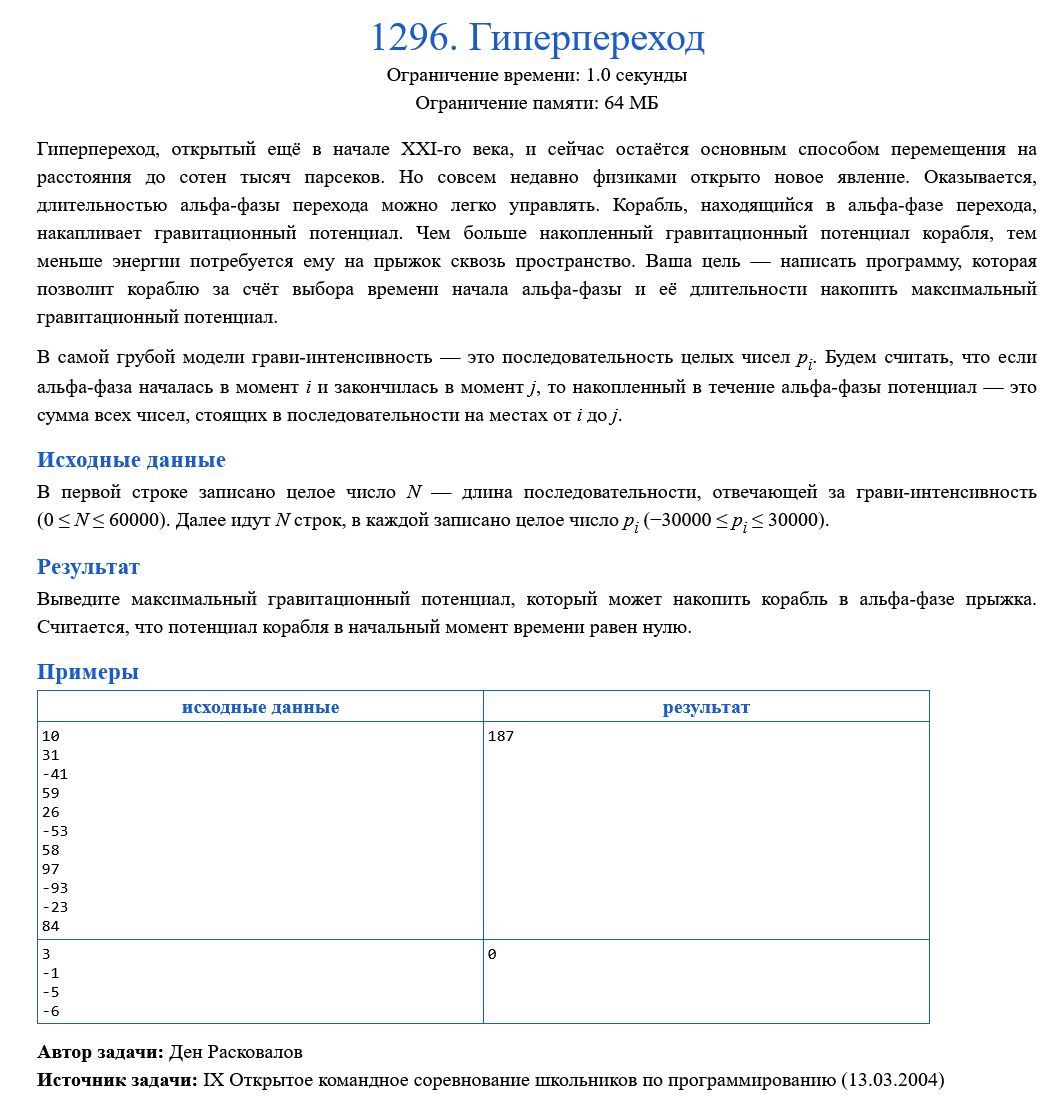
\includegraphics[width=0.9\linewidth]{pic/task_1296.png}}
\caption{Условие задачи 1296.}
\end{figure}

\subsection{Основная идея}
Задача сводится к поиску максимальной суммы подпоследовательности последовательности $p_i$.

\subsection{Краткое описание алгоритма}
\textbf{1. Входные данные:} целое число$N$ -- длина последовательности, отвечающей за грави-интенсивность $(0 \leq N \leq 60000)$. Дальше идут $N$ строк, в каждой записано целое число $p_i$ $ (-3000 \leq p_i \leq 30000)$.\\
\textbf{2.} Считываем построчно числа и записываем их сумму в переменную$cur\_sum$.\\
\textbf{3.} На каждой итерации цикла проверяем, что текущая сумма неотрицательна, иначе объявляем ее нулевой.\\
\textbf{4.} На каждой итерации проверяем, что максимальная сумма не меньше текущей, иначе присваиваем значение текущей суммы максимальной.\\
\textbf{5. Выходные данные:} целое неотрицательное число -- максимальный гравитационный потенциал, который накопит корабль в альфа-фазе прыжка.


\subsection{Листинг}

\begin{center}
\begin{lstlisting}[label=some-code,caption={Исходный код для 1296}]
#include <iostream>


int main() {
    int n;
    std::cin >> n;

    // task to search substring with max sum
    int max_sum = 0;
    int cur_sum = 0;

    for (int i = 0; i < n; ++i) {
        int cur_p;
        std::cin >> cur_p;

        cur_sum += cur_p;
        cur_sum = cur_sum < 0 ? 0 : cur_sum;
        max_sum = max_sum < cur_sum ? cur_sum : max_sum;
    }
}

\end{lstlisting}
\end{center}

\subsection{Результат}
\begin{figure}[h]
\center{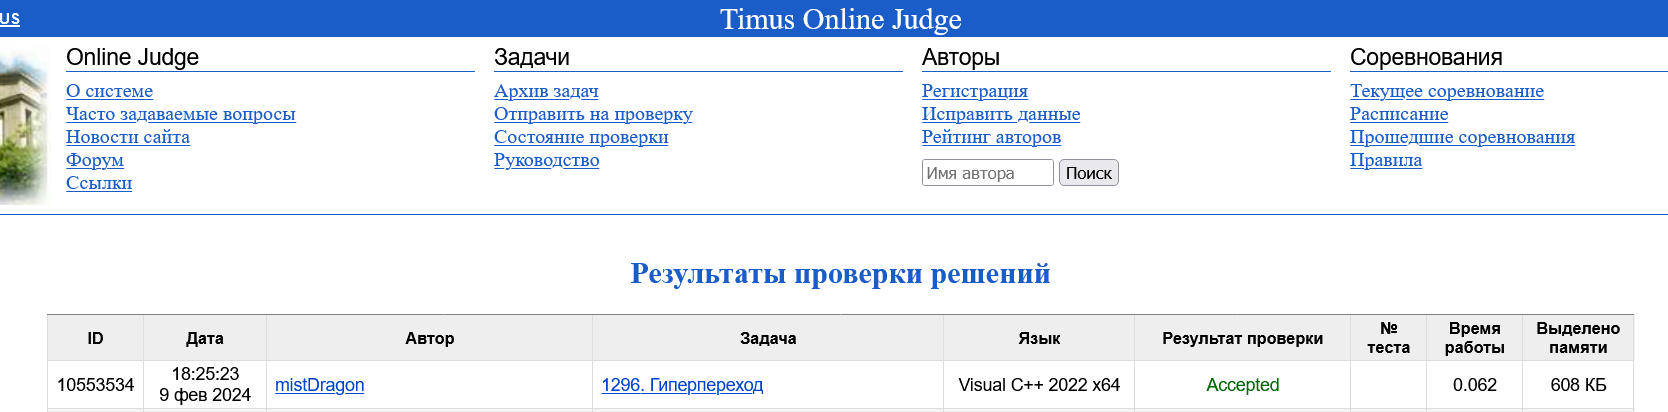
\includegraphics[width=0.9\linewidth]{pic/screen_1296.png}}
\caption{Результат отправки задачи 1296.}
\end{figure}


\newpage
\section{Задача 1494}

\begin{figure}[h]
\center{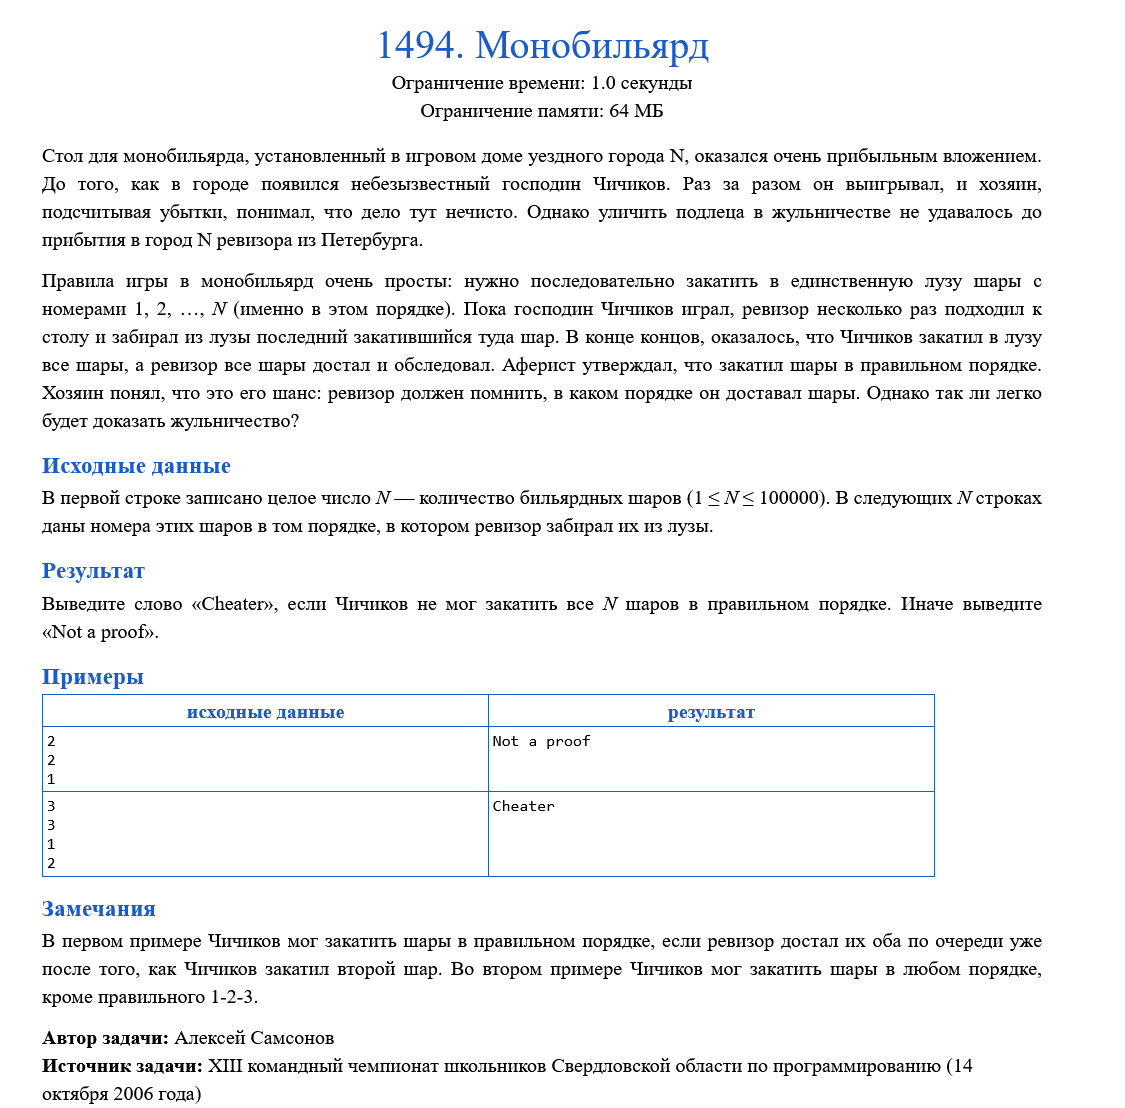
\includegraphics[width=1\linewidth]{pic/task_1494.png}}
\caption{Условие задачи 1494.}
\end{figure}


\subsection{Основная идея}
Основная идея состоит в том, чтобы на каждом шаге итерации проверять, является текущая подпоследовательность обратной с шагом 1.

\subsection{Краткое описание алгоритма}
\textbf{1. Входные данные:} количество шаров -- целое число $n$, такое что $(1 \leq n \leq 100000)$. В следующих $n$ строках даны номера этих шаров в том порядке, в котором ревизор забирал их из луны. \\
\textbf{2.} Введем переменные $temp$ -- отвечает за максимальный встреченный номер шара, тип $int$; $cheater$ -- отвечает за то, уличен ли Чичиков в читерстве, тип $bool$. Так же объявим $stack\_of\_balls$ -- помогает нам проверять, корректно ли загнаны в лунку шары. \\
\textbf{3.} При вводе каждого нового номера шара, проверяем, больше ли он $temp$, если, да, тогда складываем в стек номера с $temp + 1$ до текущего номера шара. Затем обновляем значение $temp$, присваивая ему значение текущего шара; иначе проверяем равенство текущего номера шара значению вершины стека, если это условие выполнено, то убираем верхний номер шара, иначе, присваеваем переменной $cheater$ значение $true$, так как получена последовательность неудовлетворяющая условиям честной игры. \\
\textbf{5. Выходные данные:} строка $"Not\,\, a \,\, proof"$ -- для случая честной игры, иначе -- $"Cheater"$ .

\subsection{Структуры данных}
В данной работе была использована структура данных \textbf{стек}. Стек сравним со стопкой книг, когда мы складываем книги первая оказывается в самом низу. Книги можно забирать только с вершины, то есть мы не можем вытаскивать книги из случайного места стопки. Чтобы достичь книги, которую мы положили первой, необходимо снять все книги, которые были сложены в стопку после нее. Выполняется принцип \textbf{First In -- Last Out (FILO)}.

\newpage
\subsection{Листинг}

\begin{center}
\begin{lstlisting}[label=some-code,caption={Исходный код для 1494}]
#include <iostream>
#include <stack>


int main() {
    int n;
    std::cin >> n;
    // special data structure stack (first in - last out)
    // helps to check order of balls
    std::stack<int> stack_of_balls;
    bool cheater = false;
    // the biggest number of ball was input
    int temp = 0;
    for (int i = 0; i < n; ++i) {
        int cur_ball;
        std::cin >> cur_ball;
        // check and update stack of the balls
        if (temp < cur_ball) {
            for (int j = temp + 1; j < cur_ball; ++j) {
                stack_of_balls.push(j);
            }
            temp = cur_ball;
        } else {
            // check if current ball is on the top of stack
            if (cur_ball == stack_of_balls.top()) {
                // update stack by pop the highest
                stack_of_balls.pop();
            } else {
                cheater = true;
            }
        }
    }

    if (cheater) {
        std::cout << "Cheater" << std::endl;
    } else {
        std::cout << "Not a proof" << std::endl;
    }
}
\end{lstlisting}
\end{center}

\subsection{Результат}
\begin{figure}[h]
\center{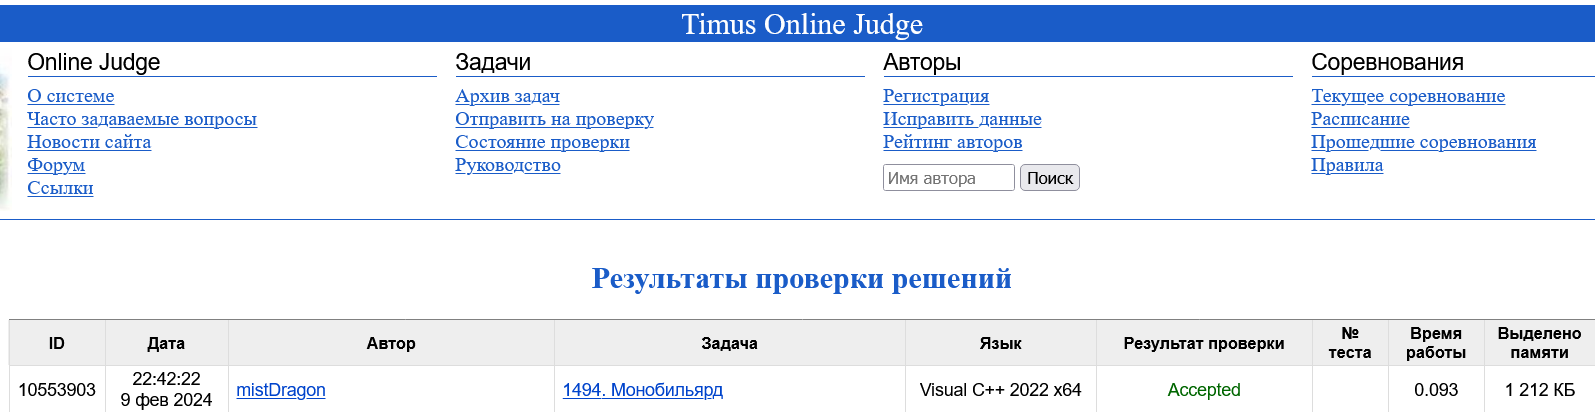
\includegraphics[width=0.9\linewidth]{pic/screen_1494.png}}
\caption{Результат отправки задачи 1494.}
\end{figure}




\newpage
\section{Вывод по работе}
В ходе выполнения данной лабораторной работы были оеализованы алгоритмы для решения задач $1296$, $1494$. Для решения задачи $1494$ была использована особая структура данных -- стек.
\end{document}













